\documentclass[compress]{beamer}
\usetheme{sthlm}

%-=-=-=-=-=-=-=-=-=-=-=-=-=-=-=-=-=-=-=-=-=-=-=-=
%        LOADING BEAMER PACKAGES
%-=-=-=-=-=-=-=-=-=-=-=-=-=-=-=-=-=-=-=-=-=-=-=-=

\usepackage{
booktabs,
datetime,
dtk-logos,
graphicx,
multicol,
pgfplots,
ragged2e,
tabularx,
tikz,
wasysym,
multirow,
float,
caption,
subcaption
}

\pgfplotsset{compat=1.8}

\usepackage[utf8]{inputenc}
\usepackage[portuguese]{babel}
\usepackage[T1]{fontenc}
\usepackage{newpxtext,newpxmath}
\usepackage{listings}

\lstset{ %
language=[LaTeX]TeX,
basicstyle=\normalsize\ttfamily,
keywordstyle=,
numbers=left,
numberstyle=\tiny\ttfamily,
stepnumber=1,
showspaces=false,
showstringspaces=false,
showtabs=false,
breaklines=true,
frame=tb,
framerule=0.5pt,
tabsize=4,
framexleftmargin=0.5em,
framexrightmargin=0.5em,
xleftmargin=0.5em,
xrightmargin=0.5em
}



%-=-=-=-=-=-=-=-=-=-=-=-=-=-=-=-=-=-=-=-=-=-=-=-=
%        LOADING TIKZ LIBRARIES
%-=-=-=-=-=-=-=-=-=-=-=-=-=-=-=-=-=-=-=-=-=-=-=-=

\usetikzlibrary{
backgrounds,
mindmap
}

%-=-=-=-=-=-=-=-=-=-=-=-=-=-=-=-=-=-=-=-=-=-=-=-=
%        BEAMER OPTIONS
%-=-=-=-=-=-=-=-=-=-=-=-=-=-=-=-=-=-=-=-=-=-=-=-=

\setbeameroption{show notes}

%-=-=-=-=-=-=-=-=-=-=-=-=-=-=-=-=-=-=-=-=-=-=-=-=
%        BEAMER COMMANDS
%-=-=-=-=-=-=-=-=-=-=-=-=-=-=-=-=-=-=-=-=-=-=-=-=


%-=-=-=-=-=-=-=-=-=-=-=-=-=-=-=-=-=-=-=-=-=-=-=-=
%
%	PRESENTATION INFORMATION
%
%-=-=-=-=-=-=-=-=-=-=-=-=-=-=-=-=-=-=-=-=-=-=-=-=

\title{Sincronização e \\coordenação}
\subtitle{DCE540 - Computação Paralela e Distribuída}
%\date{\small{\jobname}}
\author{\texttt{Iago Carvalho}}
\institute{\texttt{Departamento de Ciência da Computação}}

\hypersetup{
pdfauthor = {Iago A. Carvalho},      
pdfsubject = {Computação Paralela e Distribuída},
pdfkeywords = {},  
pdfmoddate= {D:\pdfdate},          
pdfcreator = {WriteLaTeX}
}

\begin{document}

\begin{frame}
\titlepage

\end{frame}

%% --------------------------------------------------------

\begin{frame}{Sincronização e coordenação}

Por sincronização, pode-se entender que
\begin{itemize}
    \item um processo aguarda a conclusão de outro
    \item ambos são executados em sincronia
    \item sincronização de dados
    \begin{itemize}
        \item garantir que os dados de dois ou mais processos são os mesmos
    \end{itemize}
\end{itemize}

\vspace{0.5cm}

Por coordenação, pode-se entender que
\begin{itemize}
    \item deve-se coordenar as interações e dependencias entre dois ou mais processos
\end{itemize}

\vspace{0.5cm}

Pode-se dizer que coordenação encapsula sincronização

\end{frame}

%% --------------------------------------------------------

\begin{frame}{Sincronização por \textit{clock}}

Uma das formas mais simples de obtermos sincronização em sistemas distribuídos é realizando sincronização por \textit{clock}
\begin{itemize}
    \item Aqui, \textit{clock} se refere a horário e não ao ciclo de \textit{clock} do computador
\end{itemize}

\vspace{0.5cm}

Em sistemas não-distribuídos, o \textit{clock} é uma ótima forma de realizar sincronização
\begin{itemize}
    \item Exemplo: \textit{make} em sistemas UNIX
\end{itemize}

\vspace{0.5cm}

Entretanto, em sistemas distribuídos, não existe necessariamente o conceito de um relógio global
\end{frame}

%% --------------------------------------------------------

\begin{frame}{Um \textit{make} em sistemas distribuídos}

\vspace{0.5cm}

\centering 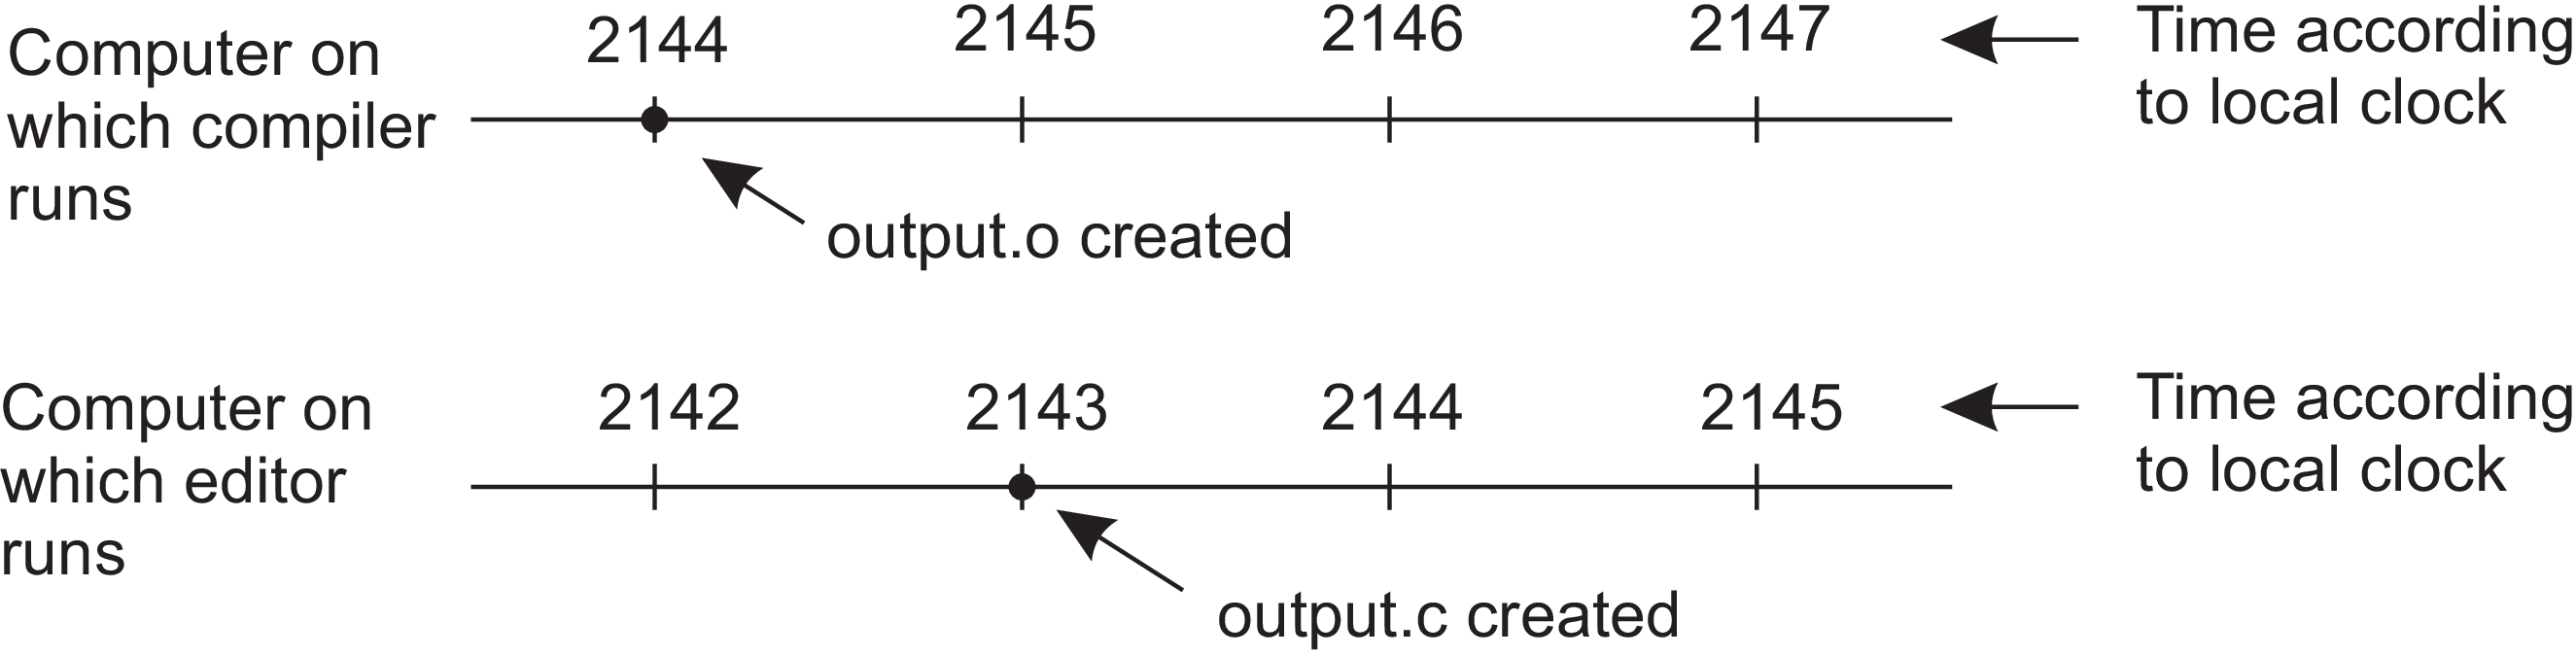
\includegraphics[width=\textwidth]{images/make.png}

\end{frame}

%% --------------------------------------------------------

\begin{frame}{\textit{Clocks} físicos}

Todo computador possui um \textit{clock} físico
\begin{itemize}
    \item um cristal de quartzo localizado na placa mãe
\end{itemize}

\vspace{0.5cm}

Este cristal é alimentado por uma bateria externa e possui uma RAM própria

\vspace{0.5cm}

Quando alvo de uma corrente elétrica, o cristal produz uma oscilação
\begin{itemize}
    \item frequência da oscilação é estável e bem definida
    \item a cada \textit{n} oscilações, gera-se uma interrupção de sistema
    \item esta interrupção conta um segundo
\end{itemize}
\end{frame}

%% --------------------------------------------------------

\begin{frame}{Sincronização de \textit{clock}}

Pode-se considerar o UTC (Universal Coordinated Time) como um \textit{clock} global

\vspace{0.5cm}

Caso um computador seja sincronizada com o UTC 
\begin{itemize}
    \item Outros computadores podem sincronizar seus \textit{clocks} com este primeiro
\end{itemize}

\vspace{0.5cm}

Seja $t$ o tempo dado pelo UTC. Além disso, seja $C_p(t)$ o tempo atual em um computador $p$. O objetivo de um algoritmo de sincronização de \textit{clock} é garantir que
$$
\forall t, \forall p, q : | C_p(t) - C_q(t) | \leq \pi,
$$
onde $\pi$ é uma medida de \textbf{precisão} mínima
\end{frame}

%% --------------------------------------------------------

\begin{frame}{Sincronização de \textit{clock}}

A precisão anterior refere-se unicamente a diferença de tempo entre dois computadores parte de um mesmo sistema distribuído.

\vspace{0.5cm}

Quando medimos a discrepância do tempo entre um computador e o UTC, estamos medindo sua \textbf{acurácia}, que é dada por

$$
\forall t, \forall p: | C_p(t) - t| \leq \alpha,
$$

onde $\alpha$ é a acurácia mínima desejada

\vspace{0.5cm}

O objetivo de algoritmos de sincronização de \textit{clock} é garantir
\begin{itemize}
    \item Precisão mínima entre os computadores de um sistema distribuído
    \item Acurácia dos \textit{clocks} de cada computador em relação ao UTC
\end{itemize}
\end{frame}

%% --------------------------------------------------------

\begin{frame}{Desvio de \textit{clock}}

Um \textit{clock} baseado em cristal de quartzo possui um desvio médio de $10^{-6}$ segundos por segundo
\begin{itemize}
    \item Equivalente a 31,5 segundos por ano, aproximadamente
\end{itemize}

Todo sistema de \textit{hardware} que faz medição de \textit{clock} possui um desvio máximo de \textit{clock} $\rho$ especificado

Seja $F(t)$ a frequência de oscilação do \textit{clock} de uma máquina em um instante $t$. Além disso, seja $F$ a frequência ideal de oscilação. Podemos dizer que o desvio de \textit{clock} de uma máquina obedece a equação

$$
\forall t: (1 - \rho) \leq \frac{F(t)}{F} \leq (1 + \rho)
$$
\end{frame}

%% --------------------------------------------------------

\begin{frame}{Desvio de \textit{clock}}

Considere o \textit{clock} de dois computadores estejam desviando-se do UTC em direções opostas
\begin{itemize}
    \item O primeiro sempre mais rápido
    \item O segundo sempre mais lento
\end{itemize}

A \textbf{precisão} destes \textit{clocks} será até de 
$$
2\rho\,\Delta t
$$

Para se garantir uma precisão $\pi$, os \textit{clocks} devem ser resincronizados pelo menos a cada 

$$
\frac{\pi}{2\rho}~~\textnormal{segundos}
$$
\end{frame}

%% --------------------------------------------------------

\begin{frame}{Network Time Protocol (NTP)}

\centering 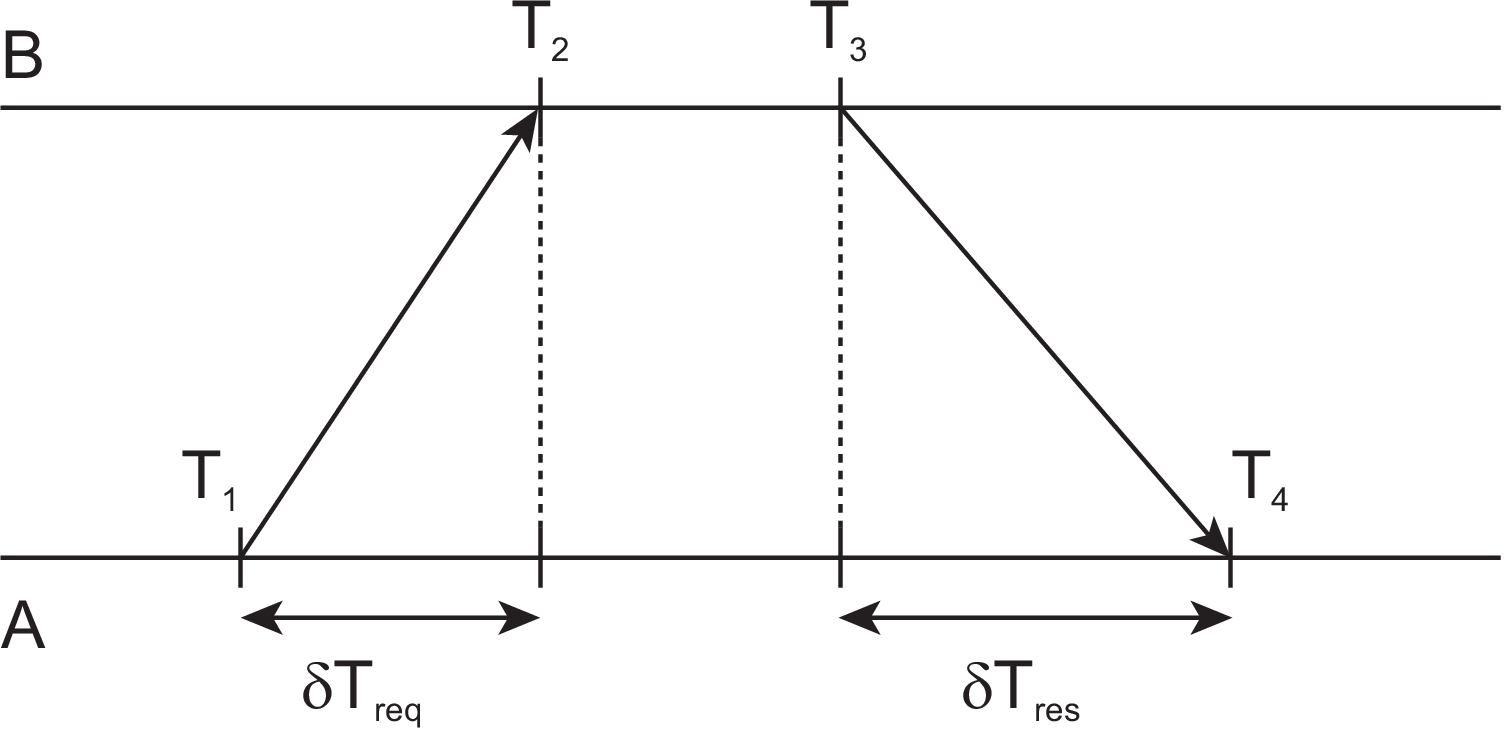
\includegraphics[width=0.7\textwidth]{images/ntp.png}

\begin{enumerate}
    \item A manda requisição para B no tempo $T_1$
    \item B recebe a requisição no tempo $T_2$
    \item No tempo $T_3$, B responde A enviando o valor $T_2$
    \item A recebe a resposta no tempo $T_4$
\end{enumerate}
\end{frame}

%% --------------------------------------------------------

\begin{frame}{Network Time Protocol (NTP)}

\centering 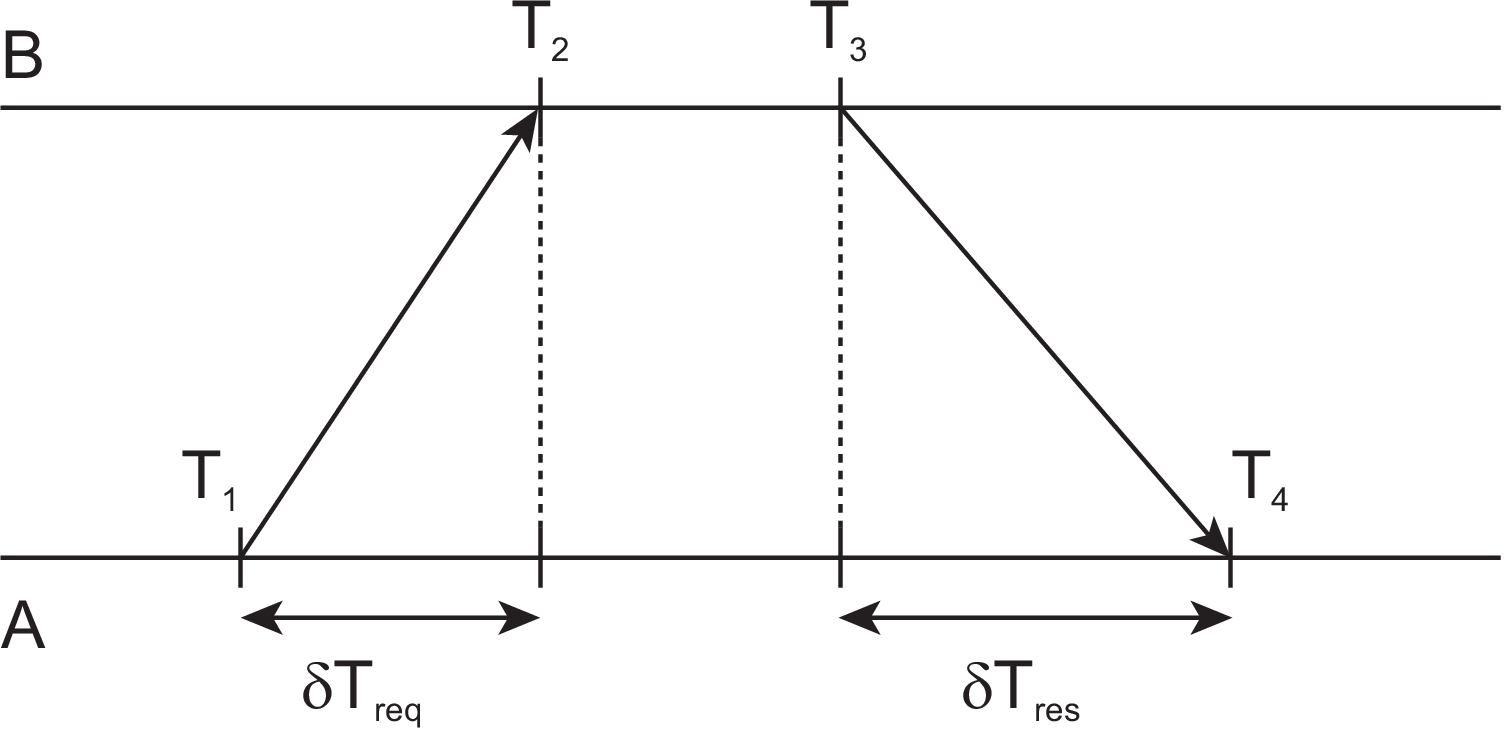
\includegraphics[width=0.7\textwidth]{images/ntp.png}

$$
\textnormal{offset } \theta = T_3 + \frac{(T_2 - T_1) + (T_4 - T_3)}{2} - T_4 = \frac{(T_2 - T_1) + (T_4 - T_3)}{2}
$$

$$
\textnormal{delay } \delta = \frac{(T_4 - T_1) - (T_3 - T_2)}{2}
$$
\end{frame}

%% --------------------------------------------------------

\begin{frame}{Algoritmo de Berkley}

Um servidor tenta continuamente atualizar os \textit{clocks} dos computadores que fazem parte de um sistema distribuído

\vspace{1cm}
 
\centering 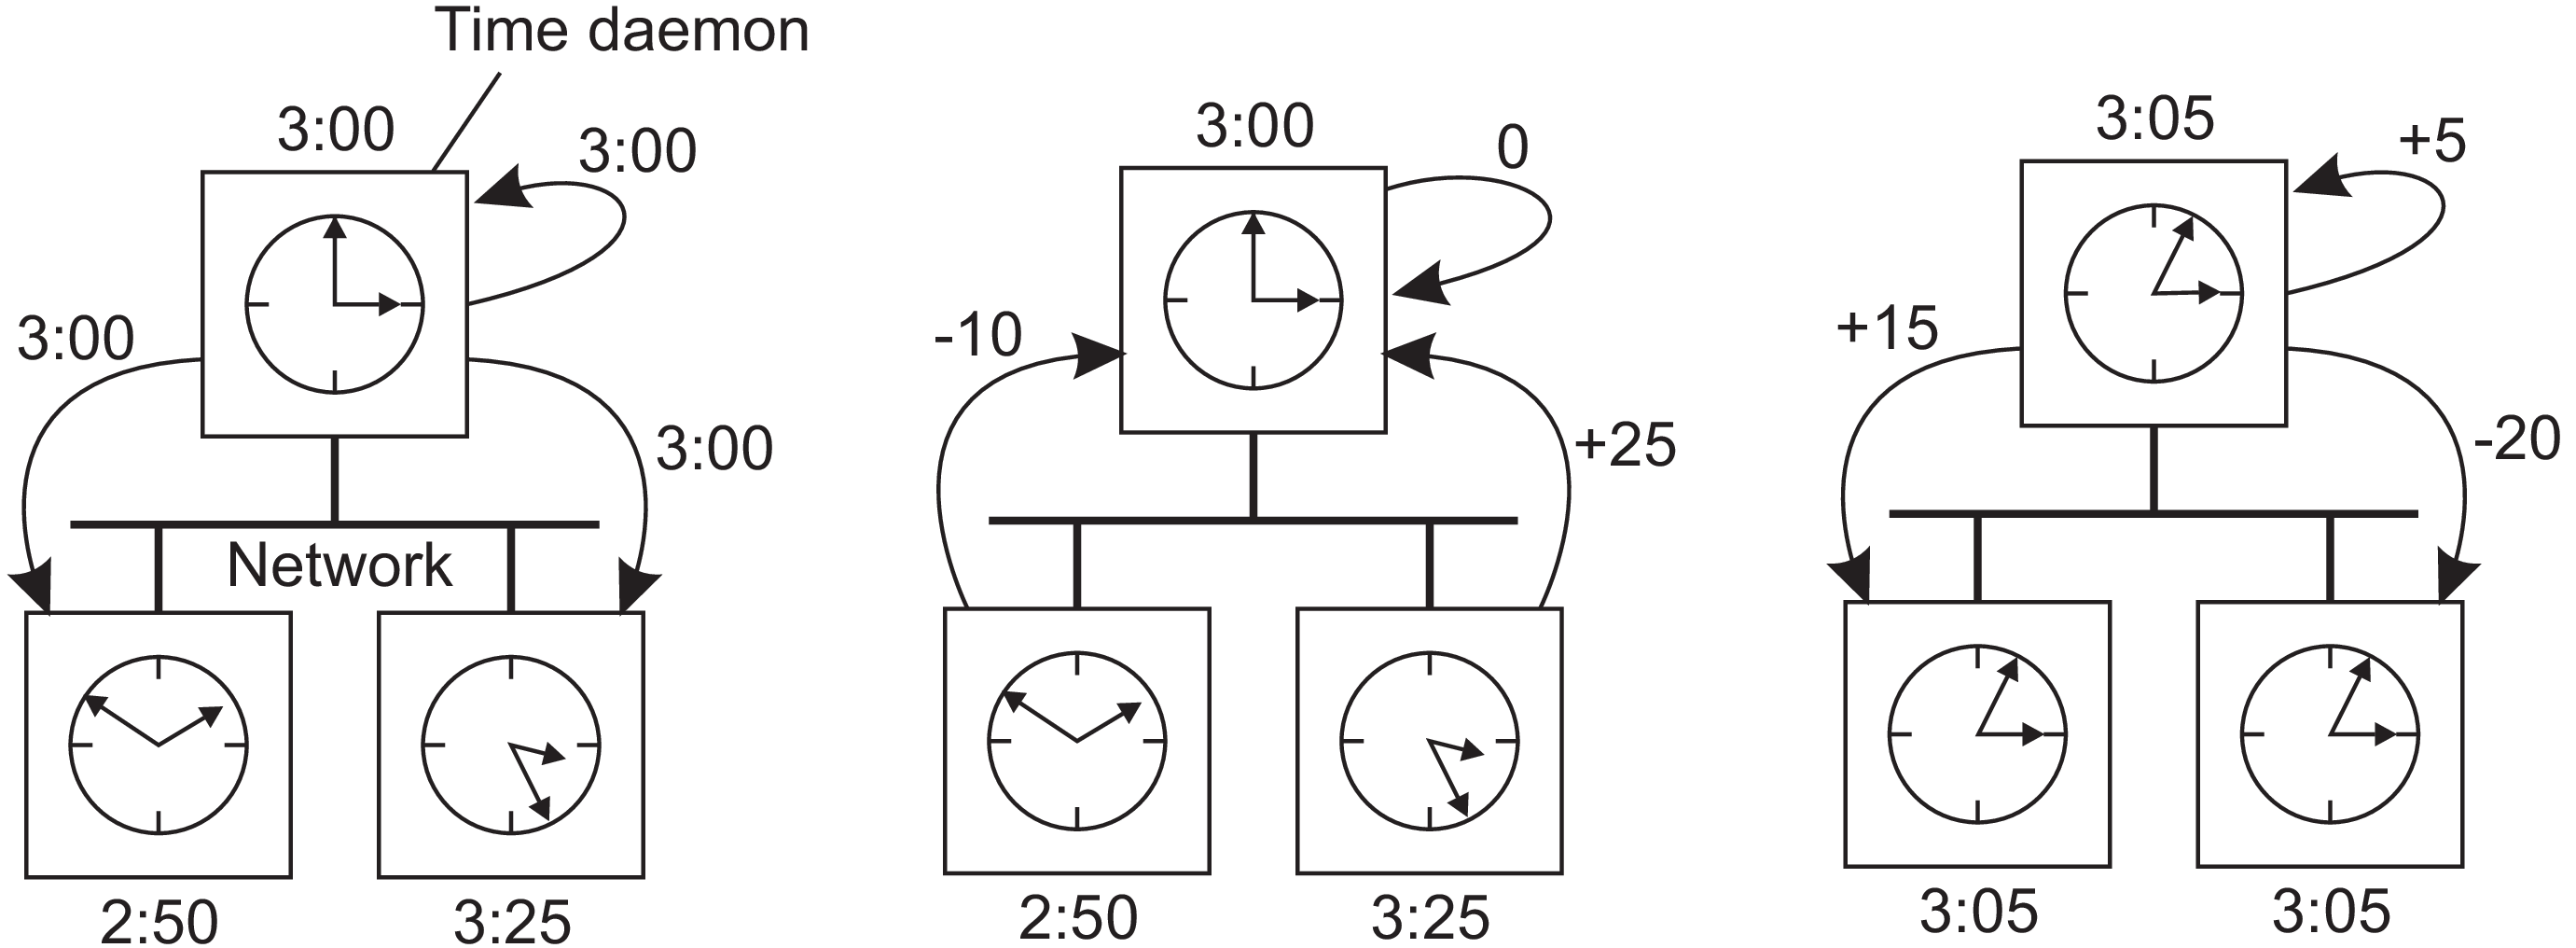
\includegraphics[width=\textwidth]{images/berkeley.png}

\end{frame}

%% --------------------------------------------------------

\begin{frame}{\textit{Clock} lógico}

\textit{Clock} lógico refere-se ao fato de que não é necessário sincronizar os \textit{clocks} das máquinas
\begin{itemize}
    \item Ao invés disso, deve-se saber somente a ordem em que os eventos no sistema ocorreram
\end{itemize}

\vspace{0.5cm}

Este esquema de sincronização também diz que não é necessário que o \textit{clock} de todas as máquinas do sistema estejam sincronizados
\begin{itemize}
    \item Só é necessário sincronizar o \textit{clock} daquelas máquinas ou dispositivos que interagem umas com as outras
\end{itemize}

\end{frame}

%% --------------------------------------------------------

\begin{frame}{\textit{Clock} lógico - Algoritmo de Lamport}

\centering 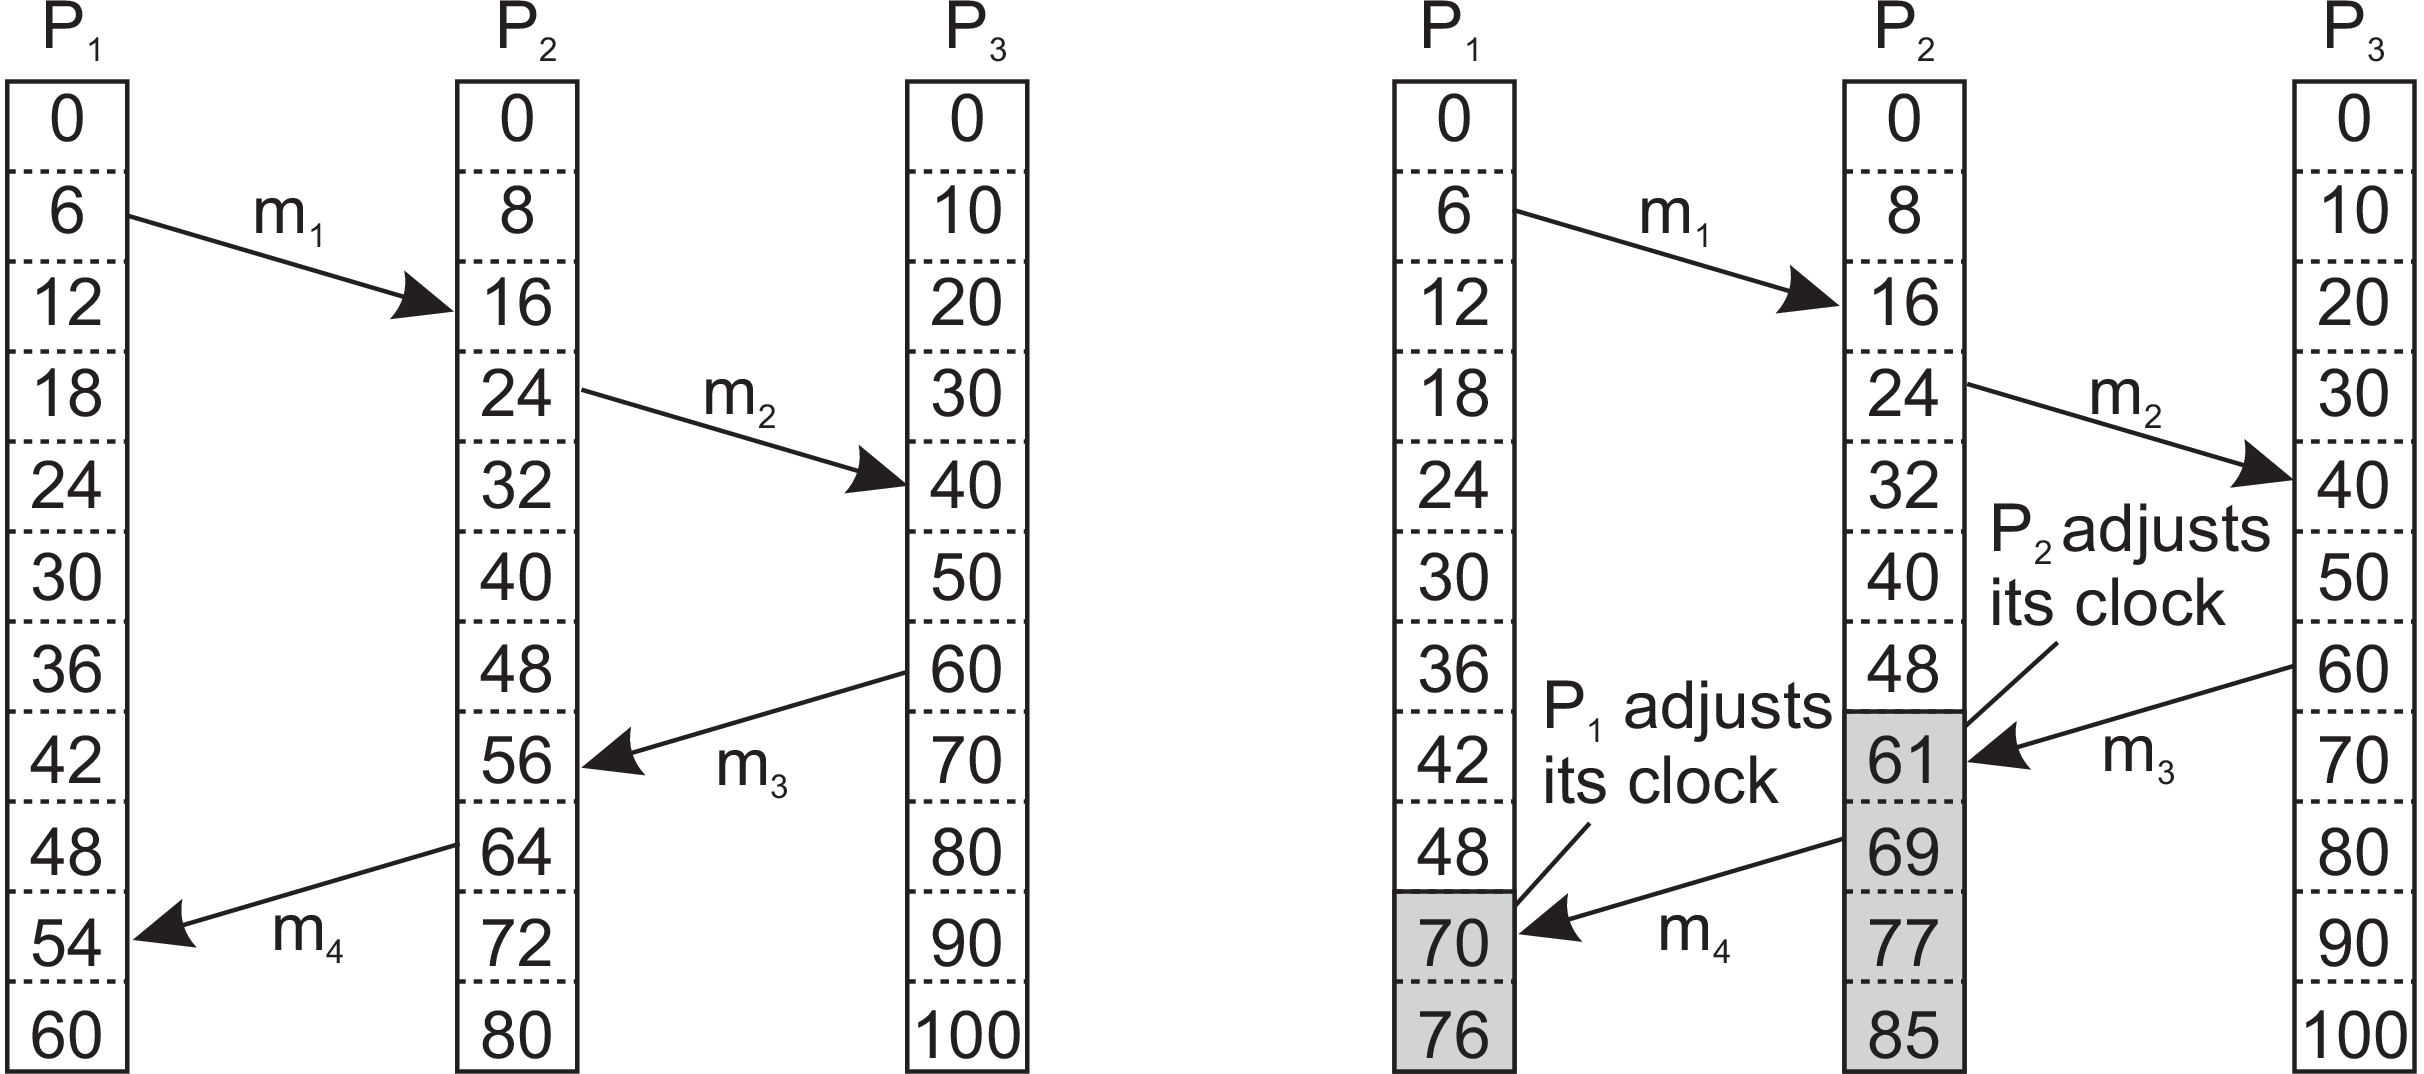
\includegraphics[width=\textwidth]{images/lamport.png}

\end{frame}

\end{document}
